\documentclass[12pt, letterpaper]{article}

\usepackage[utf8]{inputenc}
\usepackage[english]{babel}
\usepackage[T1]{fontenc}
\usepackage{graphicx}
\usepackage{tikz}
\usepackage{subfig}

\renewcommand{\baselinestretch}{1.3}

\begin{document}

\begin{titlepage}

\begin{center}
	\large{EC336: Embedded Systems}\\
	\huge{\textbf{Interfacing Display Devices}}\\
	\large{Arvind S Kumar (15EC106), Pavan M (15EC13),\\ Samarth B (15EC143), Sripathi M (15EC149)}\\
	\large{15 August 2018}
\end{center}	

\begin{figure}[!h]
	\centering
	\includegraphics[scale=0.8]{/home/sripathi/GitHub_Repositories/NITK_Emblem.png}
	\label{fig:NITKEmblem}
\end{figure}	
\begin{center}
	
\huge{Submitted to:}\\
\begin{large}
Prof. Ramesh Kini M, Prof. Arulalan Rajan\\
Department of Electronics and Communication Engineering\\
NITK, Surathkal
\end{large}

\end{center}

\end{titlepage}

\section{Goal of the Lab}

The aim of this lab was to interface the chosen microcontroller with display devices such as LEDs, 7-segment displays and LCD displays. The micro controller chosen by our group is TI's MSP430G2.

\section{Components Used}

For this lab the components used are :

\begin{itemize}
	\item MSP430 microcontroller
	\item LEDs
	\item 2.2 k$\Omega$ resistors
	\item 2 7-segment displays
	\item LCD displays
\end{itemize}

\section{Board Details}

Some of the features of the MSP430 are -

\begin{itemize}
	\item 16-bit RISC architecture
	\item Von-Neumann architecture
	\item Upto 16 MHz clock frequency
	\item Low power consumption and five power saving modes
	\item 16 general purpose registers
	\item 10-bit ADC
	\item Supports SPI, I2C, UART and USB interfaces
	\item Has 10 GPIO pins divided as two ports (8-bit and 2-bit respectively)
\end{itemize}
	
\begin{figure}[t]
	\centering
	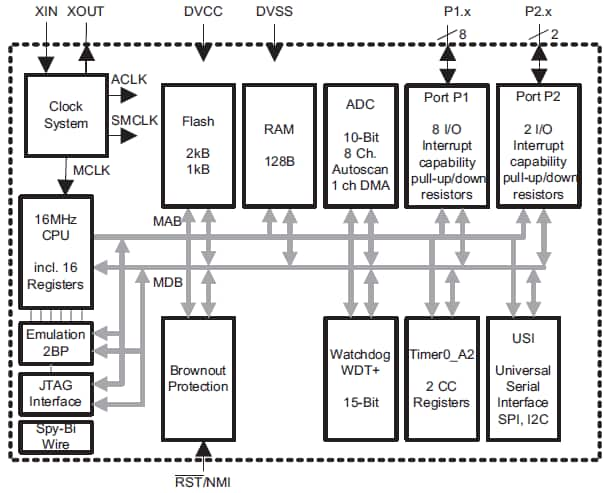
\includegraphics[scale=0.8]{/home/sripathi/GitHub_Repositories/Embedded-Systems/LatexFiles/InterfacingDisplayDevices/msp430g2231-ep-ti.png}
	\caption{MSP430 Architecture}
	\label{fig:architecture}
\end{figure}

\begin{figure}[t]
	\centering
	\subfloat[fig:board][Board]{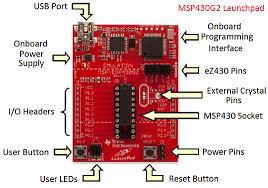
\includegraphics[scale=0.8]{/home/sripathi/GitHub_Repositories/Embedded-Systems/LatexFiles/InterfacingDisplayDevices/board_msp430.jpeg}}
		\subfloat[fig:pindiagram][Pin Diagram]{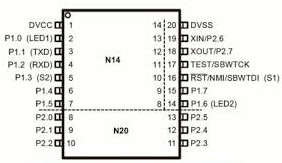
\includegraphics[scale=0.8]{/home/sripathi/GitHub_Repositories/Embedded-Systems/LatexFiles/InterfacingDisplayDevices/pinout_msp430.jpeg}}
		\caption{Board details}
		\label{fig:board}
\end{figure}

	

\end{document}